\section{Transformation Passes}

\subsection{Basic Block Extraction}

Basic Block extraction is a very simple transformation pass that given a basic block in a function it extracts
that basic block into a new function, a call instruction to the new function is then inserted inplace of the basic block.
The changes are illustrated by Figure 1 on the top of the following page.

\begin{figure}[t]
  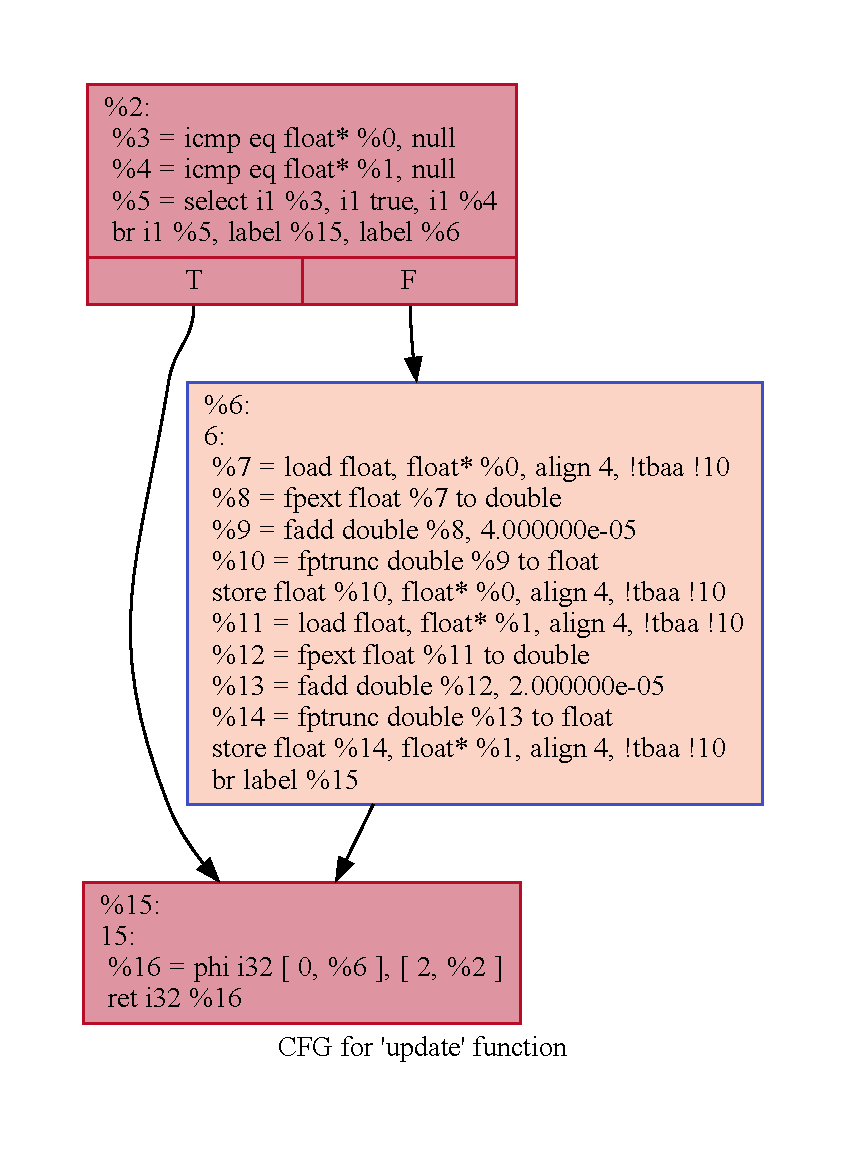
\includegraphics[width=0.5\textwidth]{./images/update.pdf}
  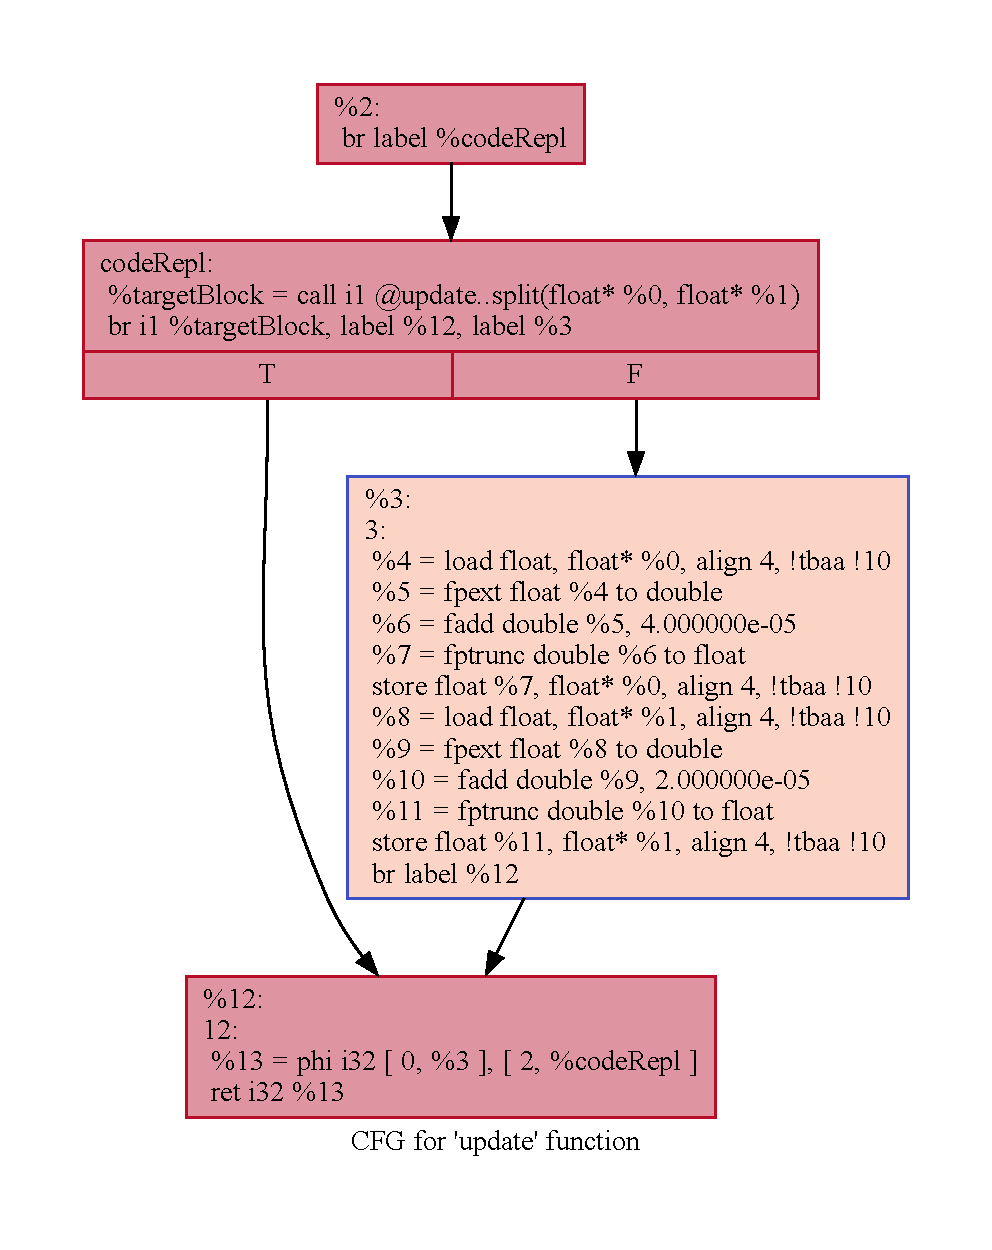
\includegraphics[width=0.5\textwidth]{./images/block-extraction-update.pdf}
  \caption{Block Extraction Transformation Pass}
\end{figure}

By itself the block extraction doesn't add much confusion to the control flow graph, if however combined with
other transformation passes, which further obfuscate the newly created function for the extracted block, it can result
in strong control flow obfuscation.

\subsection{Operation Substitution}

Operation substitution is another simple transformation pass that substitutes an instruction into a sequence
of instructions which ultimately end up with the same result.

This method is also known as Mixed Boolean-Arithmetic expressions. The MBA expressions were collected from \cite{ollvm, mba-exp} with
some variations.

The used substitutions are listed below where A is the result B, C are the operators of the expresion and R is
a random value.

\begin{center}
\begin{tabular}{|l|}
  \hline
  AND Substitution $a = b \land c$ \\
  \hline
  $a = (b \oplus \neg c) \land b$ \\
  $a = \neg(\neg b \lor \neg c) \land (r \lor \neg r)$ \\
  $a = (\neg b \lor c) - (\neg b)$ \\
  \hline
  XOR Substitution $a = b \oplus c$ \\
  \hline
  $a = (b \oplus r) \oplus (c \oplus r)$\\
  $a = (\neg b \land c) \lor (b \land \neg c)$\\
  $a = (b \lor c) - (b \land c)$\\
  $a = (\neg b \land r \lor b \land \neg r) \oplus (\neg c \land r \lor c \land \neg r)$\\
  \hline
\end{tabular}
\end{center}

\begin{center}
\begin{tabular}{|l|}
  \hline
  OR Substitution $a = b \lor c$ \\
  \hline
  $a = (b \land c) \lor (b \oplus c)$ \\
  $a = (b \land \neg c) + c$ \\
  $a = [(\neg b \land r) \lor (b \land \neg r) \oplus (\neg c \land r) \lor (c \land \neg r)] \lor $ \\
  $[\neg(\neg b \lor \neg c) \land (r \lor \neg r)]$ \\
  \hline
  Sub Substitution $a = b - c$ \\
  \hline
  $a = b + (-c)$ \\
  $a = b + r$; $a = a - c$; $a = a - r$  \\
  $a = b - r$; $a = a - c$; $a = a + r$  \\
  \hline
  Add Substitution $a = b + c$ \\
  \hline
  $a = b - (-c)$ \\
  $a = -(-b + (-c))$ \\
  $a = b + r$; $a = a + c$; $a = a - r$ \\
  $a = b - r$; $a = a + c$; $a = a + r$ \\
  $a = (b \land c) + 2 * (b \oplus c)$ \\
  $a = (b \land c) + (b \lor c)$ \\
  \hline
\end{tabular}
\end{center}

In addition to the $Add$ $substitution$ there is also a special substitution for 8-bit integers.

     a = $(((b \oplus c) + 2 * (b \land c)) * 39 + 23) * 151 + 111$

\subsection{String Obfuscation}

When obfuscating strings, you can't avoid reconstructing the original string because at some point you will have to work with it, for example before comparing it to other strings, printing it via print, etc.
Thus, string obfuscation plays an important role in static analysis, but it can be broken by watching the execution of the program until the transformation is reversed and working with the original string.

This transformation pass is implemented by making use of Mealy machines as described in Chapter 4.5.3 of \cite{ss-chpt4}

Consider the string $Hello$ for which the following state machine was build.

\begin{center}
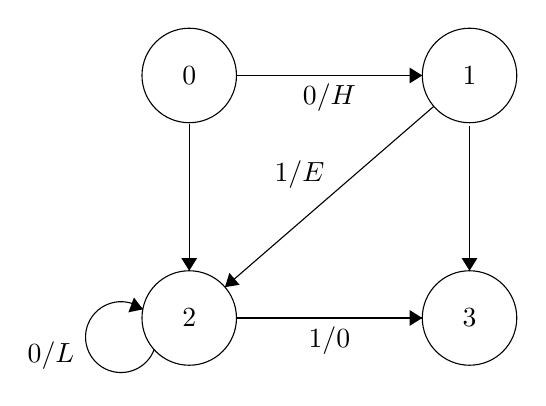
\begin{tikzpicture}[scale=0.2]
\tikzstyle{every node}+=[inner sep=0pt]
\draw [black] (24.1,-21.4) circle (3);
\draw (24.1,-21.4) node {$0$};
\draw [black] (41.9,-21.4) circle (3);
\draw (41.9,-21.4) node {$1$};
\draw [black] (24.1,-36.8) circle (3);
\draw (24.1,-36.8) node {$2$};
\draw [black] (41.9,-36.8) circle (3);
\draw (41.9,-36.8) node {$3$};
\draw [black] (27.1,-21.4) -- (38.9,-21.4);
\fill [black] (38.9,-21.4) -- (38.1,-20.9) -- (38.1,-21.9);
\draw (33,-21.9) node [below] {$0/H$};
\draw [black] (39.63,-23.36) -- (26.37,-34.84);
\fill [black] (26.37,-34.84) -- (27.3,-34.69) -- (26.65,-33.94);
\draw (31.1,-28.61) node [above] {$1/E$};
\draw [black] (21.876,-38.796) arc (-20.35775:-308.35775:2.25);
\draw (16.83,-39.17) node [left] {$0/L$};
\fill [black] (21.16,-36.25) -- (20.59,-35.5) -- (20.24,-36.44);
\draw [black] (27.1,-36.8) -- (38.9,-36.8);
\fill [black] (38.9,-36.8) -- (38.1,-36.3) -- (38.1,-37.3);
\draw (33,-37.3) node [below] {$1/0$};
\draw [black] (41.9,-24.6) -- (41.9,-33.8);
\fill [black] (41.9,-33.8) -- (42.4,-33) -- (41.4,-33);
\draw [black] (24.1,-24.5) -- (24.1,-33.8);
\fill [black] (24.1,-33.8) -- (24.6,-33) -- (23.6,-33);
\end{tikzpicture}
\end{center}

In the binary it would be replace with the sequence $01001$, when decoding the sequence into the original
string we need some information to reconstruct the string from the state machine, for this we use two arrays.

\lstset{language=C} % Set the language to C
\lstset{basicstyle=\ttfamily} % Set the basic style as monospaced
\begin{lstlisting}
// transitions to nodes
int next[][2] = {
    {1, 2},
    {3, 2},
    {2, 3}
};
// printable chars
char out [][2] = {
    {'H', 'q'},
    {'t', 'E'},
    {'L', 'O'}
};
\end{lstlisting}

We always start from node $0$, for the transition from that node we look at the outgoing edges and take the next bit from the generated sequence which
is also $0$. $next[0][0]$ this yields the next node which is $1$ and the character $out[0][0]$ which is 'H'. This is repeated until the bit sequence is consumed.

\subsection{Opaque Predicates}

Most of the implemented transformation passes in this paper rely on opaque predicates. As described in Chapter 4.3.1 in \cite{ss-chpt4}
opaque predicates are simply expressions that are either opaquely true or opaquely false.

\begin{figure}
  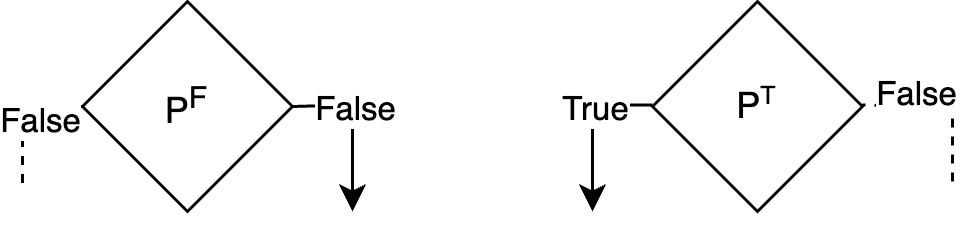
\includegraphics[width=1\textwidth]{./images/predicates.jpeg}
  \caption{Opaque Predicates}
\end{figure}

The predicates used as the condition shouldn't be to easy to break. For example this opaquely true predicate $x\oplus x ==0$ is easy to break
and most decompilers (and also optimazation passes) wouldn't have a problem deducing the result.

Thus in the transformation pass when inserting predicates we decided to use more numerical expressions which
work $\forall x \in \mathbb{Z}$

\begin{center}
\begin{tabular}{|l|}
  \hline
  Opaquely True predicates \\
  \hline
  $(x \land 1 == 0) \lor [3 * (x^{2} + x)] \bmod 2 == 0$\\
  \hline
  $(x \land 1 == 1) \lor (x^{2} + x) \bmod 2 == 0$ \\
  \hline
  $(2x + 2)*(2x) \bmod 4 == 0 \lor (x^{2} + x) \bmod 2 == 0$ \\
  \hline
  $3*(x^{2} + x) \bmod 2 == 0 \land (x^{2} + x) \bmod 2 == 0$ \\
  \hline
  $(x^{2} + x) \bmod 2 == 0 \land (2x+2)(2x) \bmod 4 == 0$ \\
  \hline
  $(x + x^{3}) \bmod 2 == 0 \land (2x + 2)(2x) \bmod 4 == 0$ \\
  \hline
\end{tabular}
\end{center}

These predicates are then used with the combination of the substitution pass to obfuscate the Loop conditions and add
bogus control flow by splitting a basic block at a random instruction as depicted in Figure 3.

\begin{figure}[b]
  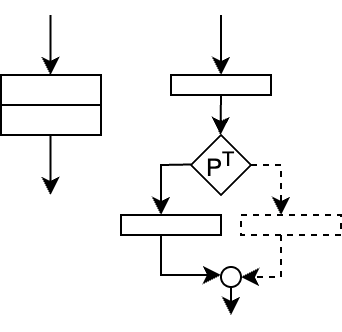
\includegraphics[width=0.5\textwidth]{./images/op.png}
  \caption{Opaque Predicates Bogus Flow}
\end{figure}

The transformation pass chooses at random whether the new block has random instructions that don't affect the program
or uses the predicate \textbf{$x \bmod 2 == 0$} to clone the block such that both block gets executed at random and in one of them
obfuscate the instructions by either adding random instructions or using the substitution pass.

This transformation pass will only transform basic blocks for which a reachable integer \footnote{A reachable integer is an integer variable that was defined up until the point when control flow reaches the basic block.} exists.

\subsection{Jump to Loop}
Jump to Loop further builds upon the opaque predicates by introducing a jump into a randomly chosen basic block
that is part of a Top-Level \footnote{Top Level Loop is the Root of the Tree of Loops nested inside it. \url{https://llvm.org/docs/LoopTerminology.html#important-notes}} Loop without
nested loops and introduces a new nested loop.

The jumped to basic block is split at a random instruction and the newly inserted
basic block filled with bogus instructions. The transformation is depicted by Figure 4.

\begin{figure}
  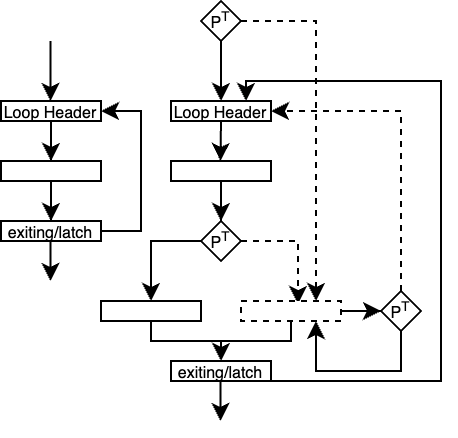
\includegraphics[width=1\textwidth]{./images/jump-to-loop.png}
  \caption{Jump To Loop}
\end{figure}

\subsection{Bogus Control Flow}

Another transformation pass that builds further upon opaque predicates. Given a basic block it first
applies the transformation described in Figure 3 it then chooses a random block from the two split blocks
continues to add bogus operations into it and proceeds to performer the same split transformation again on that chosen block

One of the latter split blocks will be chosen as the loop latch and a branch to the original basic block will be added,
forming a loop from the created transformations, this process is depicted in Figure 5.

\begin{figure}
  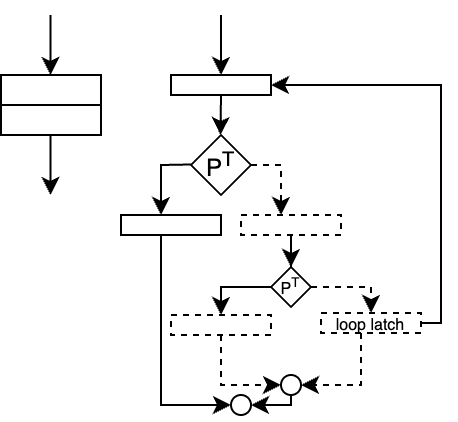
\includegraphics[width=1\textwidth]{./images/bogus-flow.png}
  \caption{Bogus Control Flow}
\end{figure}

\subsection{Function Merging}

Generally, programmers write functions to abstract away logic of a program
into a single unit that can be looked at independently from other logic of that program, making it easier to understand and read the code.

Function merging, as described in Chapter 4.6.1 of \cite{ss-chpt4}, is the exact opposite of that, we merge functions into a single function and replace all occurrences of the merged function
from the program and replaced them with the new function, this is known as abstraction breaking.

To illustrate the transformation pass consider this program.

\lstset{language=C++} % Set the language to C
\lstset{basicstyle=\ttfamily} % Set the basic style as monospaced
\begin{lstlisting}

string rand_string() {
    return to_string(rand());
}

int add(int first, int second) {
    return first + second;
}

int main() {
    int result = add_two(1, 2);
    cout << result << '\n';

    string str = rand_string();
    cout << str << '\n';
}

\end{lstlisting}

After applying the transformation pass the program will look as follows

\lstset{language=C++} % Set the language to C
\lstset{basicstyle=\ttfamily} % Set the basic style as monospaced
\begin{lstlisting}
void merged(int case, string *res,
int first, int second, int* res2) {
    switch (case) {
     case 0:
         *res = to_string(rand());
     case 1:
         *res2 = first + second;
    }
}

int main() {
    int result;
    merged(1, NULL, 1, 2, &result);
    cout << result << '\n';

    string str;
    merged(0, &str, 0, 0, NULL);
    cout << str << '\n';
}
\end{lstlisting}

\subsection{Integer Literals Obfuscation}

As with string literals, integer literals occur very frequently in a binary and information can be deduced by understanding
in what context that given integer literal is being used. Obfuscating integer literals is a bit harder as we are working with compile-time
constants and thus further optimization passes after our transformation pass could "optimize" the obfuscation away.

In \cite{YANSOllvm} I've stumbled upon an idea, that the constant obfuscation pass in that project is using, which I've liked
and thus decided to base my solution on it as well.

The idea is that we replace the integer constant with a multiplication of two carefully chosen values. The first is a randomly chosen
odd integer and the second is the modular inverse of that odd integers multiplied with the constant we want to obfuscate.

Finding the modular inverse of an odd number can be achieved with this function, explanations can be found in \cite{odd1, odd2}

\lstset{language=C++} % Set the language to C
\lstset{basicstyle=\ttfamily} % Set the basic style as monospaced
\begin{lstlisting}
uint64_t mod_inv(uint64_t x) {
    uint64_t y = (3 * x) ^ 2;
    y = y * (2 - y * x);
    y = y * (2 - y * x);
    y = y * (2 - y * x);
    y = y * (2 - y * x);
    return y;
}
\end{lstlisting}

The multiplication $ odd * (mod\_inv(odd) * constant)$ will at runtime yield the original constant. This core idea has been further obfuscated
where the operands of the multiplication are XORed with random operations that cancel out and yield the original operand.

The obfuscation of a constant after this transformation pass have the following structure

$(A \oplus ... \oplus odd \oplus ...) * (B \oplus ... \oplus mod\_inv(odd) * constant \oplus ...)$

\subsection{Branch Function Obfuscation}

The idea in Chapter 4.3.5 in \cite{ss-chpt4}, was that unconditional branch instructions would be replaced by a call to a
"branch function" that would overwrite the return address on the stack by computing a new return address from values stored in an array.

The implementation of this would be a bit tricky at the IR level in LLVM, as the assembly instructions may not be compatible for every platform,
I've thus opted out and modified the implementation.

For every function an array will be created where the addresses of each basic block within that function will be stored.
Then, two "branch functions" will be generated that calculate the return address based on the provided argument.

\lstset{language=C++} % Set the language to C
\lstset{basicstyle=\ttfamily} % Set the basic style as monospaced
\begin{lstlisting}
int8* bf(int32 *n) {
  int64 idx = map((int64)(*n));
  return &T[idx];
}

int64 map(int64 n) {
  // R is a random generated number
  return R ^ n;
}

\end{lstlisting}

At the start of the function, the created arrays will be populated by the addresses
of the basic blocks within that function.

\lstset{language=C++} % Set the language to C
\lstset{basicstyle=\ttfamily} % Set the basic style as monospaced
\begin{lstlisting}
// This is done for every
// Basic Block in that function.
K = R ^ idx;
T[map(K)] = &BlockAddress;
\end{lstlisting}

The value of K, will be generated by the transformation pass and will be a constant.

Then the replacement of branch instructions is done with an indirect branch instruction that receives the address to jump to by
calling the $bf()$ function. The argument to that function depends on whether the branch instruction being replaced is
conditional or not.

If it's conditional the branch instruction

\lstset{language=C++} % Set the language to C
\lstset{basicstyle=\ttfamily} % Set the basic style as monospaced
\begin{lstlisting}
br cond ? &BlockAddress_1:
          &BlockAddress_2;
\end{lstlisting}

Will be replaced by

\lstset{language=C++} % Set the language to C
\lstset{basicstyle=\ttfamily} % Set the basic style as monospaced
\begin{lstlisting}
K_1 = R ^ idx_1;
K_2 = R ^ idx_2;
N = cond ? K_1 : K_2;
br bf(N ^ (K_1 ^ K_2));
\end{lstlisting}

The XOR operations will cancel out and only the index into the array will be left.

Unconditional branch instructions are replaced with conditional branch instructions by using an opaquely true predicate.
The true case continue with the original Basic block and the false case has a back reference to the block itself forming a loop.
This conditional branch instruction is then modified with the same steps as above.

At a higher abstraction the changes can be imagined as

\lstset{language=C++} % Set the language to C
\lstset{basicstyle=\ttfamily} % Set the basic style as monospaced
\begin{lstlisting}
int f(int64 n) {
  if (n % 2 == 0) {
    return 2;
  } else if (n % 3 == 0) {
    return 3;
  }
  return 0;
}
\end{lstlisting}

\lstset{language=C++} % Set the language to C
\lstset{basicstyle=\ttfamily} % Set the basic style as monospaced
\begin{lstlisting}
int f(int64 n) {
  T[map(R ^ 0)] = &if-part;
  T[map(R ^ 1)] = &else-part;
  T[map(R ^ 2)] = &endif;
  T[map(R ^ 3)] = &ret;
  int result;
  goto bf(R ^ 0);
if-part:
  if (n % 2 == 0)
    result = 2;
    N = cond ? (R^3) : (R^0);
    goto bf(N^(R^0)^(R^3));
else-part:
  else if (n % 3 == 0)
    result =  3;
    N = cond ? (R^3) : (R^1);
    goto bf(N^(R^1)^(R^3));
endif:
    result = 0;
    N = cond ? (R^3) : (R^2);
    goto bf(N^(R^2)^(R^3));
ret:
    return result;
}
\end{lstlisting}

\subsection{Function Call Obfuscation}

Function call obfuscation works on the same principle as the branch function but instead of replacing branch instructions
call instructions are replaced.

The following example illustrates the transformation pass at a higher abstraction.

\lstset{language=C++} % Set the language to C
\lstset{basicstyle=\ttfamily} % Set the basic style as monospaced
\begin{lstlisting}
int add(int a, int b) {
  return a + b;
}
int f(int64 n) {
  int a = add(1, 2);
  int b = add(3, 4);
  printf("%d\n", a);
  printf("%d\n", b);
  return a + b;
}
\end{lstlisting}

\lstset{language=C++} % Set the language to C
\lstset{basicstyle=\ttfamily} % Set the basic style as monospaced
\begin{lstlisting}
int f(int64 n) {
  T[map(R ^ 0)] = (int*)(&add);
  T[map(R ^ 1)] = (int*)(&add);
  T[map(R ^ 2)] = (int*)(&printf);
  T[map(R ^ 3)] = (int*)(&printf);

  // retype and call
  int a =
  ((int (*)(int, int)))(T[map(R ^ 0)])
  (1, 2);

  int b =
  (int (*)(int, int))(T[map(R ^ 1)])
  (3, 4);

  // retype and call
  (int (*)(const char*, ...))
  (T[map(R ^ 2])("%d\n", a)

  (int (*)(const char*, ...))
  (T[map(R ^ 3)])("%d\n", b)

  return a + b;
}
\end{lstlisting}

\subsection{Control Flow Flattening}

This transformation pass implements two solutions for control flow flattening. The first is based on of Chapter 4.3.2 from \cite{ss-chpt4} also
described in \cite{ollvm}, using a switch to decide which block within the switch statement should be executed next.

The second is purely based on indirect branching, using aliasing to obfuscate the control flow.

The idea of control flow flattening is to destroy the control flow of a function. Any branching, looping or jumping is
flattened to make the original control flow hard to follow. The transformation pass is best illustrated by looking at the
transformation in Figure 7 and Figure 8 and comparing them to the orignal flow in Figure 6.

\begin{figure}[t]
  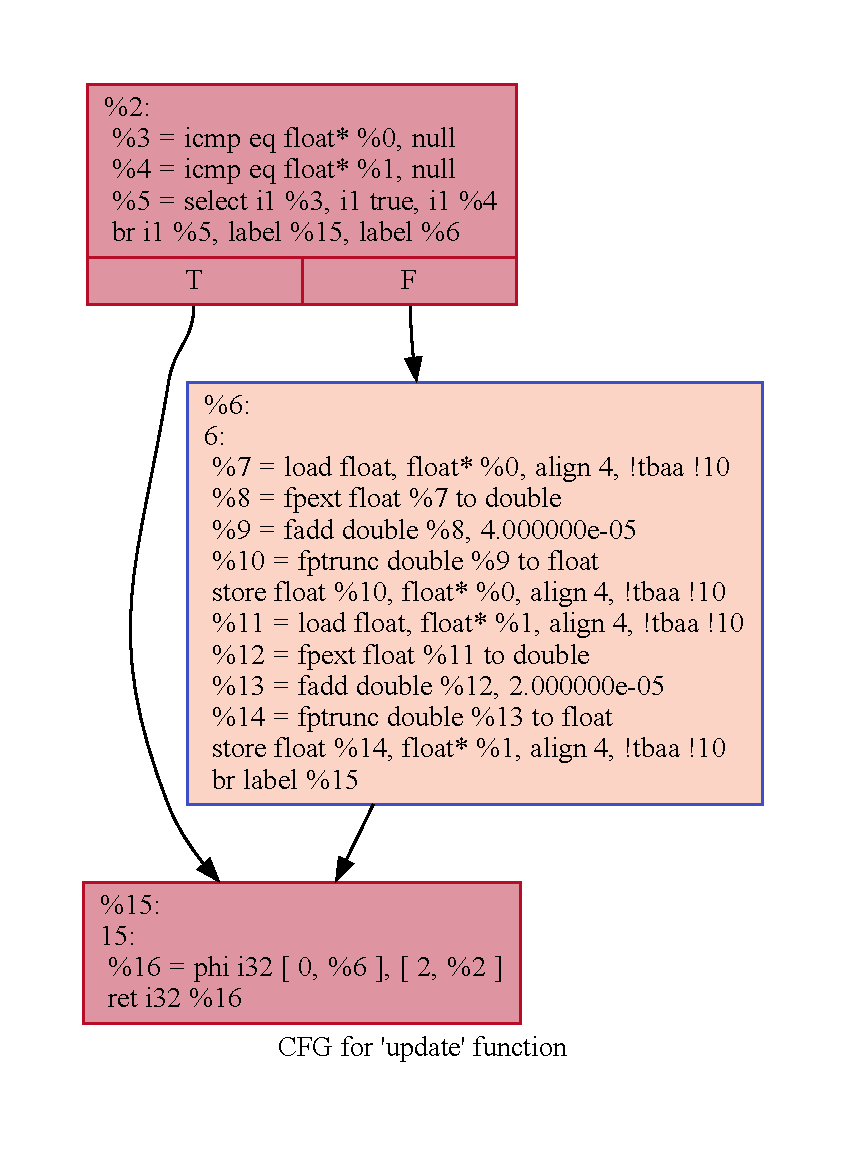
\includegraphics[width=1\textwidth]{./images/update.pdf}
  \caption{Original Function Flow}
\end{figure}

\begin{figure}[t]
  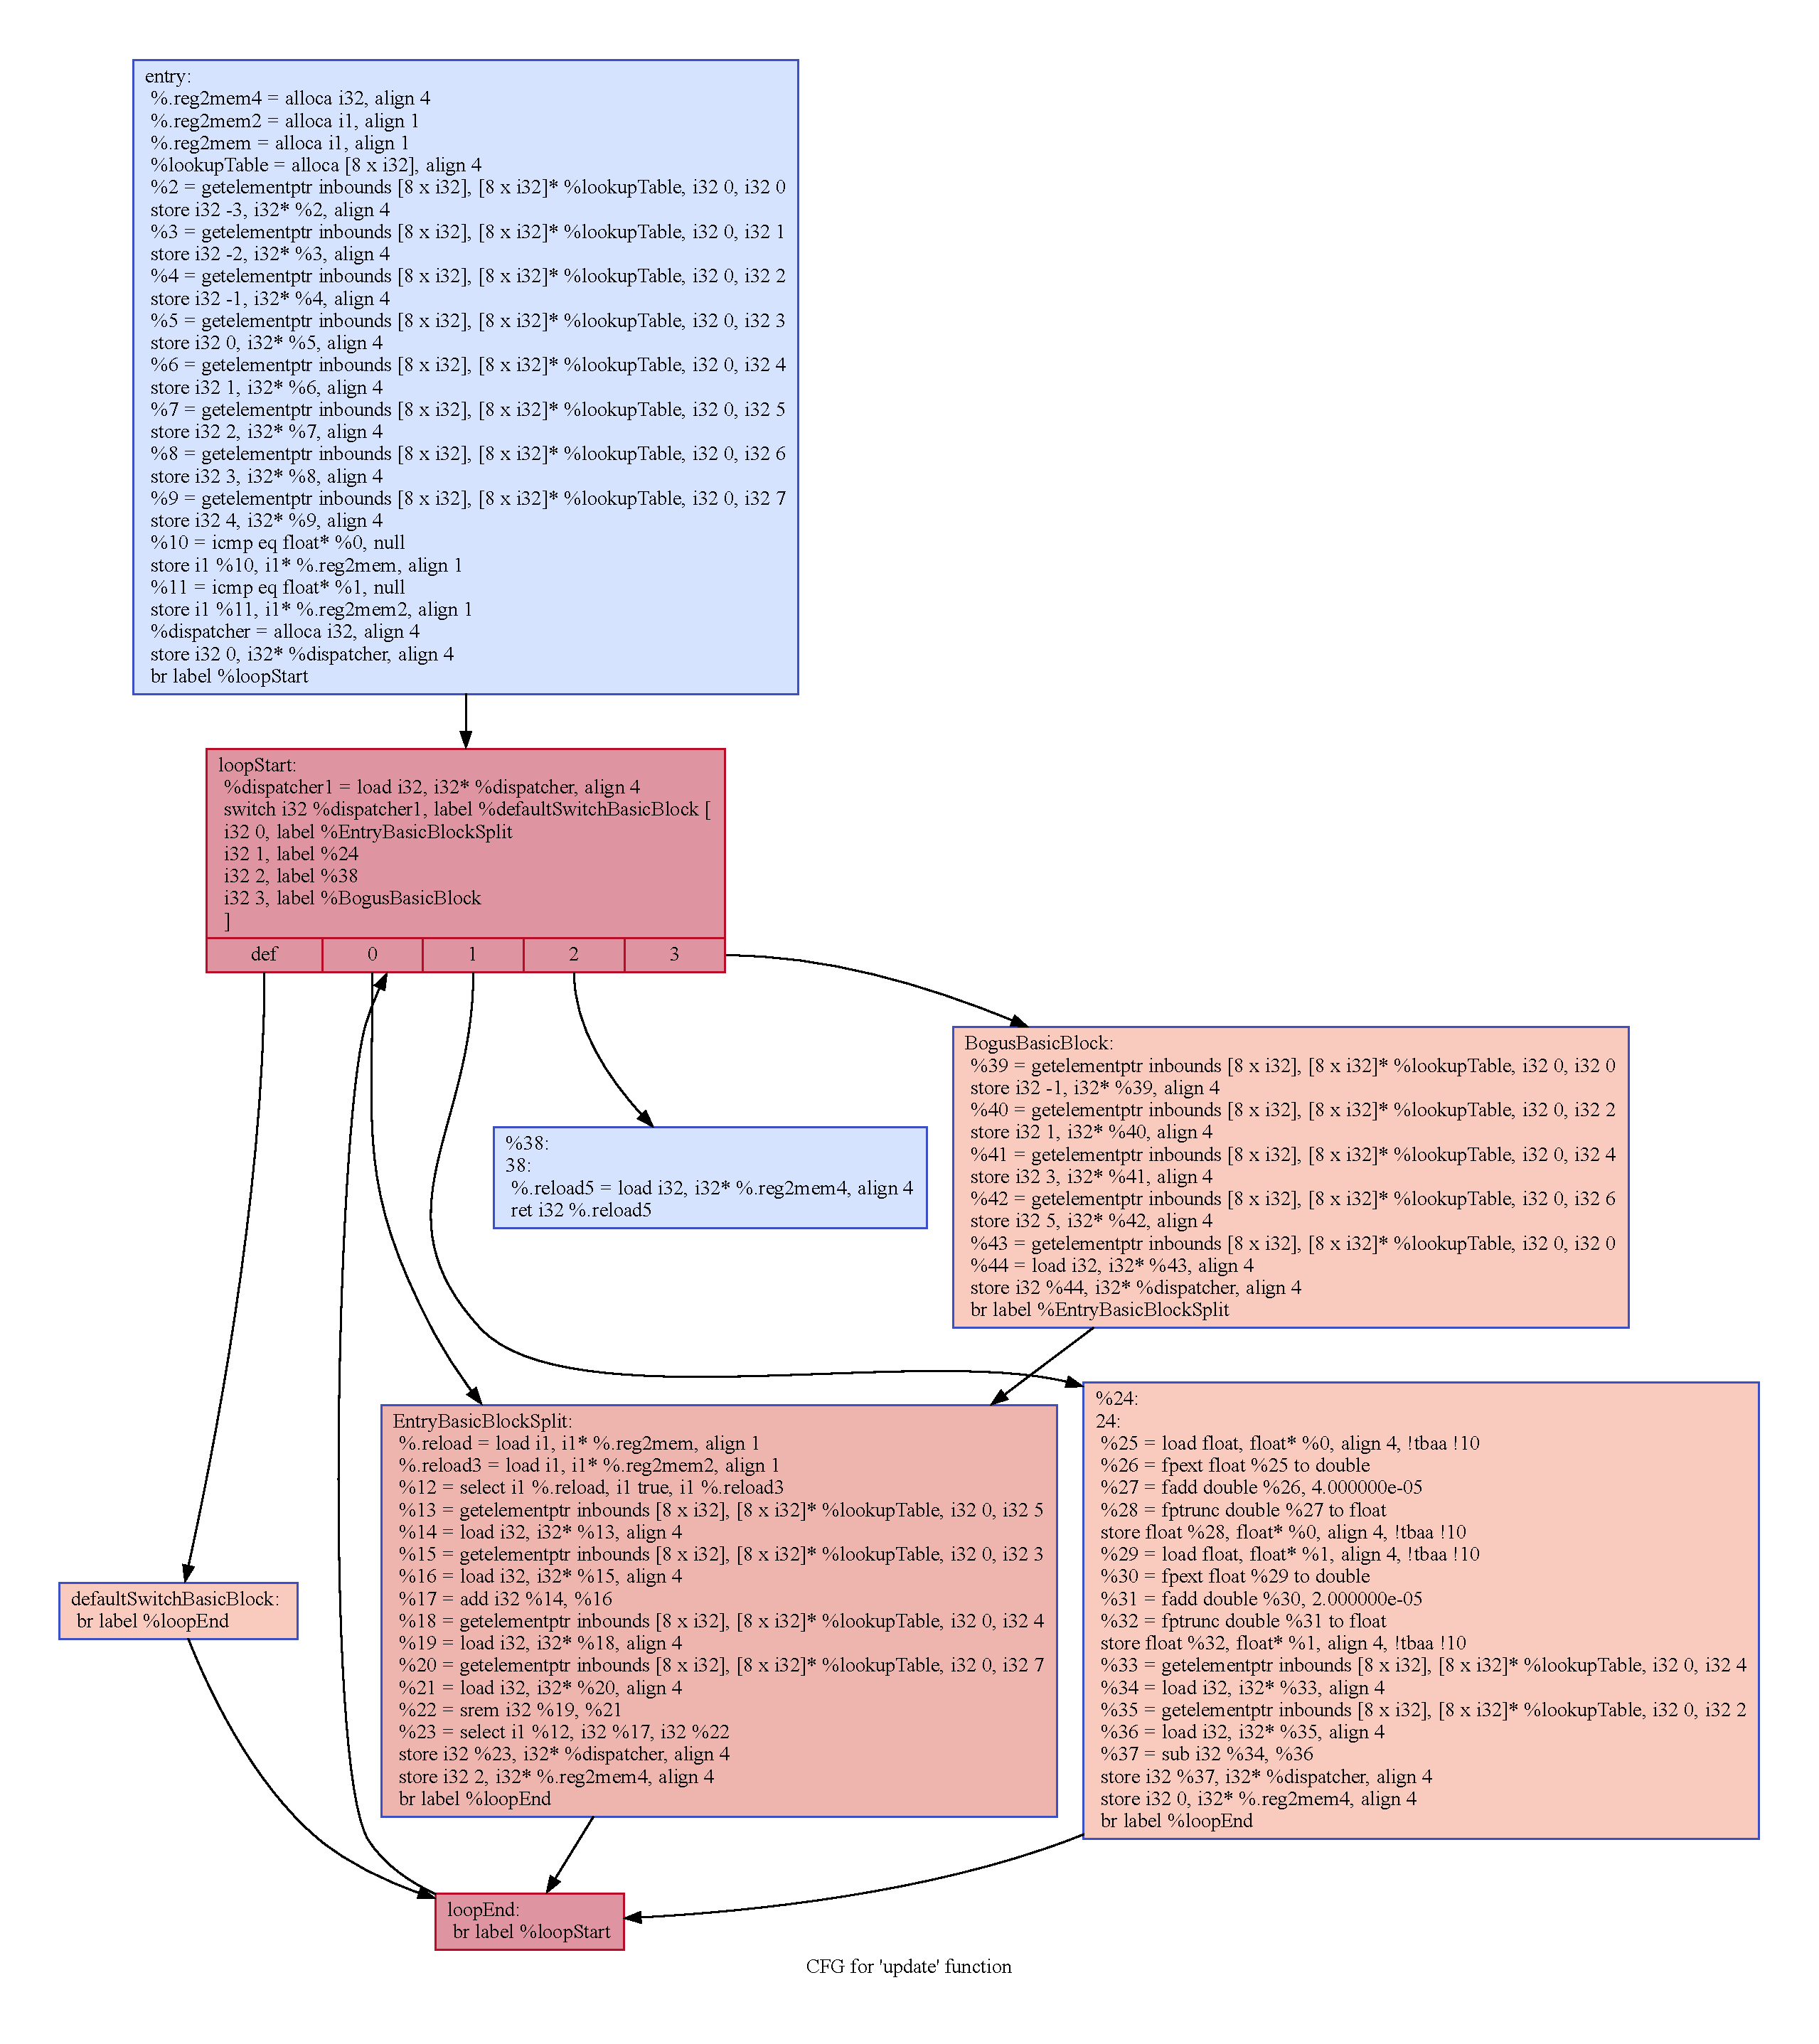
\includegraphics[width=1\textwidth]{./images/update_switch.pdf}
  \caption{Control Flow Flattening Switch}
\end{figure}

\begin{figure}[t]
  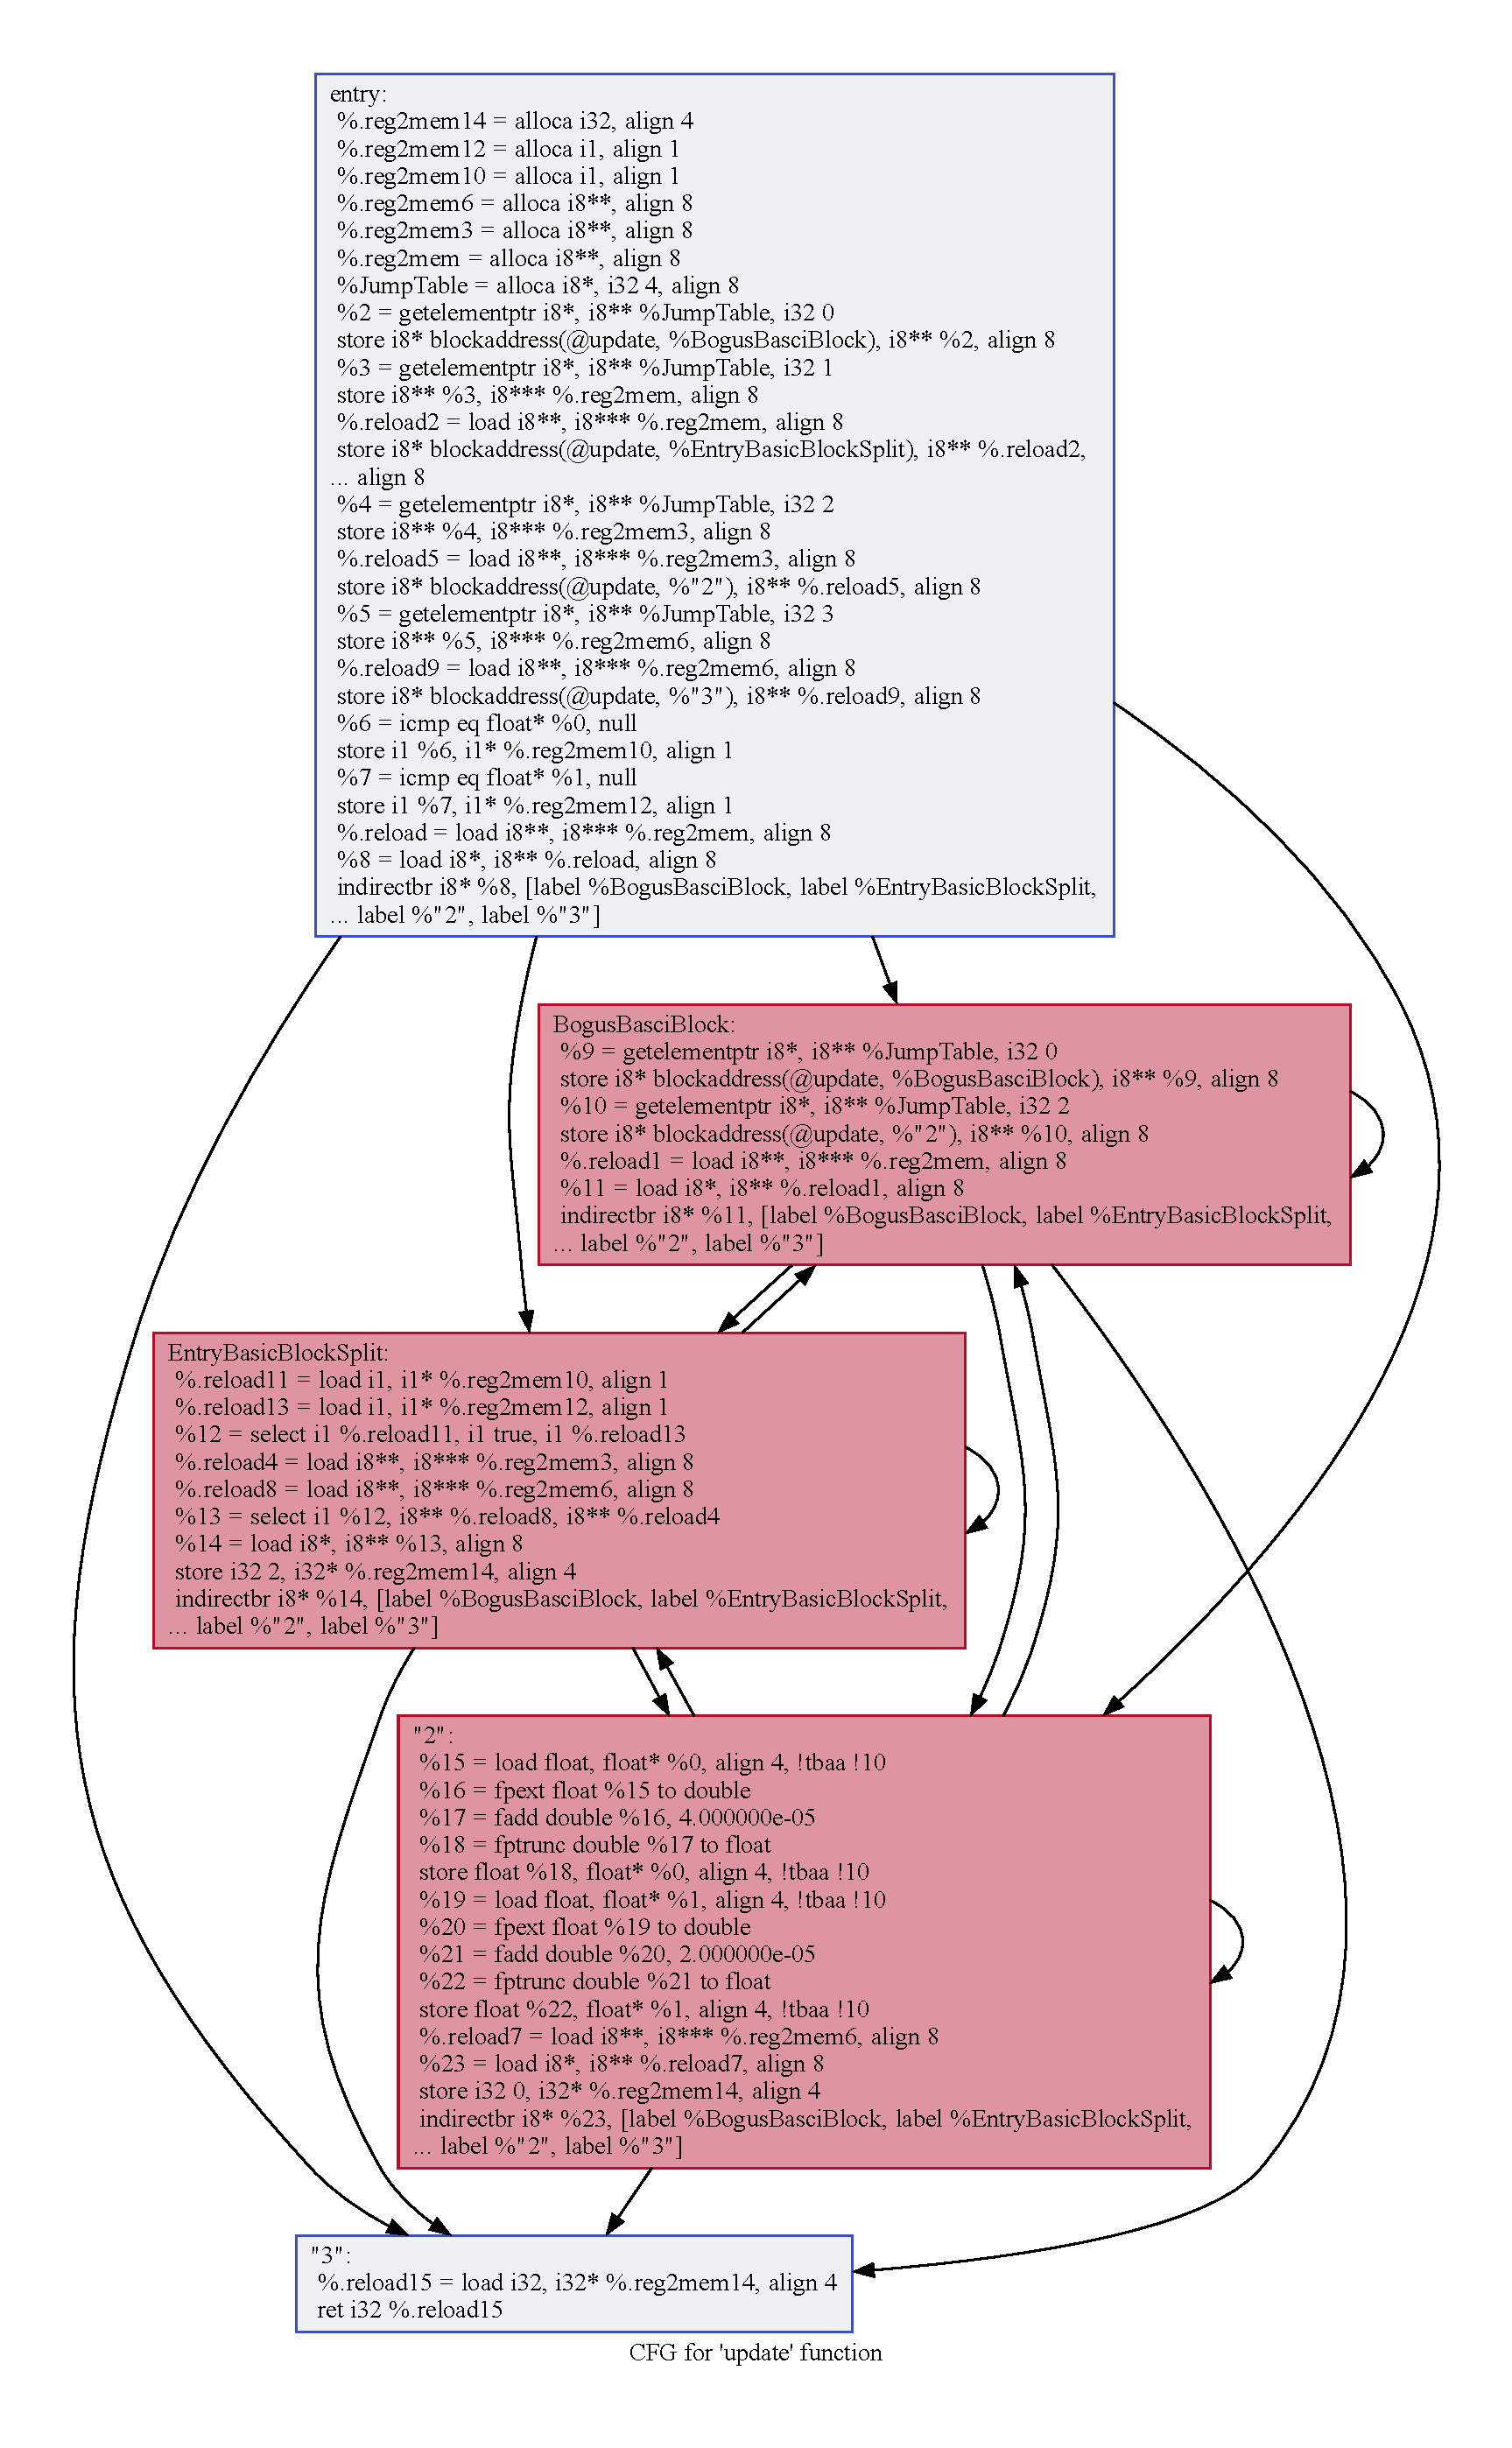
\includegraphics[width=0.8\textwidth]{./images/update_alias.pdf}
  \caption{Control Flow Flattening Aliasing}
\end{figure}

The former version uses an lookup array from which calculations are made to get the next block to be executed, addition,
subtraction and modulus is used when calculating the switch case number.

The latter version uses a lookup table where addresses are stored, it calculates the index into that lookup table to get the address to which it should jump
next.